\chapter{Introduction}

The \textit{first step} of any control problem is tipically the derivatin of a \textbf{mathematical model} for the plant to be controlled that without loss of generality is a \textbf{mechatronic system}. This is the most critical step because, assuming that we use physics laws:
\begin{itemize}
    \itemsep-0.1em
    \item We use \textit{simplifying assumptions}; 
    \item The value of the physical parameters involved in the equations (eg. mass, friction coefficients...) are not exactly known.
\end{itemize}
This fact is critical since \textit{standard} approaches to controller design are \textbf{model based}, in the sense that the controller is designed by strongly relying on the mathematical model used to describe the mechatronic system under study. Clearly the neglection of some aspects, will result in a neglection of state variables! For example for certain problems the assumption of \textit{rigid body} is satisfactory only under certain conditions.
\textbf{How to solve this problem?} If we compare the two common approaches for designing a controller (state space or  frequency description) the one based on frequency is much more able to face the problem of uncertainty.\\
In general, we can say that a controller is \textbf{robust} if it keeps good performances under the assumption of \textit{uncertain description}. For this reason we need a \textbf{robust description} of the plant that, roughly speaking, is made up of a \textbf{nominal model} and by a model for the \textbf{uncertainty}{\footnote{
    This can be modeled in an \textit{unstructured} or \textit{structured} way.
}}. Once such a model is derived we can apply some \textit{robust control techniques} for designing a controller  ($\mathcal{H}_{\infty}$, $\mu$-synthesis...)\\

In order to deal with the presence of the uncertainty and to overcome the limitations related to the first principle modeling approach we will focus on \textbf{System Identification (SysId)} (Part I)  and \textbf{Direct Data Driven Controller design (DDDC)} (Part II).

\section{Mathematical modeling of dynamical systems}
Since we have discussed about the importance of the mathematical model, now we can give an overview of the approaches one can track. 
\subsection{White-Box modeling \textit{(first principles)}} The models deriving from \textbf{white-box approach} are obtained by applying the first principle of physics and all the physical phenomena involved in the equation, also all the \textit{physical parameters} involved in the equation are \textbf{assumed to be exactly known}. The main idea which is useful to stress is that here \textbf{we know everything including the physical parameters}. 

\subsection{Gray-Box modeling}
They are models based on equations obtained (again) by applying first principles, but this time the parameters entering the equations are not exactly known and so an estimation procedure from experimantally collected data is needed. 

\subsection{Black-Box modeling}
In this case the structure of the equation is selected by the user on the basis of some "general" \textbf{a-priori information} on the system physics (eg. linearity). The parameters involved in the equation of the black-box model are then estimated/computed by using experimentally collected data. In general the parameter of a black box model do not have any \textit{physical meaning}.

\subsection{Some comments on the three approaches}
White-box models are not very useful in practice, where is very irrealistic the fact of having the knowledge of everything! Instead, more interesting is the comparison between \textbf{Gray-box} and \textbf{Black-Box} models. In both cases we have \textit{some information} (physical insights) and use the data in order to estimate the parameters themselves.

In \textbf{gray-box modeling} the structure of the equations is not selected by the user since it is forced by the first principle approach. For this reason in general the equations of a gray-box will depend in a \textbf{possibly complx nonlinear} way from the physical parameters to be estimated.

\subsubsection{Example 1 (GRAY-BOX)}
Let us assume that we know the plant to be modeled is an LTI one. You will remember that in the state-space representation, one can represent a dynamical system as:
\begin{equation*}
    \begin{aligned}
        \dot{x}(t)=Ax(t)+Bu(t)\\
        y(t)=Cx(t)+Du(t)
    \end{aligned}
\end{equation*}
If we look inside the $A$ matrix for example we can find:
\begin{equation*}
    A=\begin{bmatrix}
        \frac{m}{k^2}&\sqrt{\beta}\\
        \alpha^2\frac{k^3}{\gamma}&\gamma^2
    \end{bmatrix}
\end{equation*}
The mathematical procedure for the estimation of the parameters will be complex since they appear in the equation in a non linear way. Then, the modeling of such a plant will become very hard. This represents the main limitation of the gray-box approach. \\

\vspace{1cm}
\noindent
On the other hand, in the \textbf{black-box approach}, we have more freedom to select the structure of the equations, especially because we do it in a \textit{more convenient way} by only exploiting some general properties derived from our physical insights.

Coming back to the example we have just seen, the matrix $A$ will be made up of four coefficients $a_{ij}$ which appear linearly in the equation. The main difference is that such coefficients do not have a physical meaning.

\section{Steps for mathematical modeling}
The procedure we have for obtaining the mathematical model  is the following:
\begin{enumerate}
    \item \textsf{\textbf{STEP 1}} Exploit available \textit{a-priori information} on the system under study to select the structure of the mathematical equations describing the Input-Output mapping. In the most general case we do not know all the state variables, from this fact we can understand that we derive an \textbf{input-output model} (equation) for the plant like the following:
    \begin{equation}
        \underbrace{y(t)}_{\textsf{output}}=
        f( \underbrace{u(t)}_{\textsf{input}}, \underbrace{\theta}_{\textsf{parameters}})
    \end{equation}
    \item \textsf{\textbf{STEP 2}} Collect Input-Output data representing the behaviour of the system under study by performing an (open-loop) experiment. In particular, we collect the output $\tilde{y}$ from the plant using as input the sequence $\tilde{u}$.
    \item \textsf{\textbf{STEP 3}} To formulate a suitable \textbf{mathematical problem} to estimate/compute the values of parameter $\theta=[\theta_1...\theta_n]^T$ in such a way that our mathematical model is going to describe the behaviour of the real system, \textbf{as well as possible (in some sense)}. A common approach is to compute the parameter by solving the following problem:
    \begin{equation} \label{eq:problem}
        \hat{\theta} = \arg\min_{\theta}{J(\theta)}
    \end{equation}
    where $\hat{\theta}$ is the vector of parameters to be estimated, while $J(\theta)$ is the functional to be minimized. Usually we take it as $J(\theta)=\Vert \tilde{y}-f(\tilde{u}, \theta)\Vert$.
    At this stage the difference between gray-box and black-box approach models comes into play, since:
    \begin{itemize}
        \item \textbf{Gray-box models} $\Longrightarrow$ $f(\tilde{u}, \theta)$ will depends by a complex nonlinear function from $\theta$ (parameters); 
        \item \textbf{Black-box models} $\Longrightarrow$ $f(\tilde{u}, \theta)$ will be selected by the user in order to depend linearly from $\theta$ (if possible) or anyway in the \textit{simplest possible way}.
    \end{itemize}
\end{enumerate}

\section{Gray-Box vs Black-Box}
We have said that in the case of \textbf{Gray-box models} in general $f(u,\theta)$ may be a \textit{nonlinear} and \textit{non convex} function of $\theta$. This imply that the problem (\ref{eq:problem}) is going to be a \textbf{non convex optimization problem}, and in this case it is not trivial to solve it, the best I can say is to find \textbf{local minima}. In some situations we could be particularly lucky, and choosing a particular initial point there is the possibility of finding  the global minimum. However there is no way to certify it! Clearly a local minima, could correspond to a bad estimate of the parameter $\theta$.

\begin{figure}[h]
    \centering
    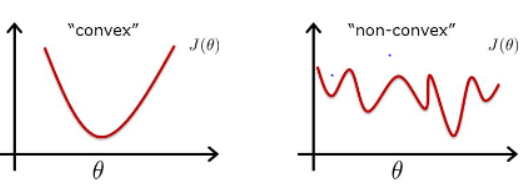
\includegraphics[scale=1]{img/cvx_nocvx.png}
    %\caption{Convex vs Non-Convex }
\end{figure}

For \textbf{Black-box} models, by selecting the parametrization of $f$ such that it could be a \textbf{convex function of $\theta$}, the problem \ref{eq:problem} becomes a \textbf{convex optimization problem}. In 1D the functional to be minimized is something similar to the one showed in the figure above. Convex functions have a  unique \textbf{global minima},there is no chance to be trapped in a local minima as in the non convex case. Clearly, waht is missed in this kind of approach is the \textit{physical meaning} of the estimated parameters. Let us give an example to better clarify this aspect: 

\subsubsection{Example (Second-order LTI system)}
Suppose that from first principles of physics we derive the following transfer function:
\begin{equation*}\label{eq:nonlinear}
    H(s)=\frac{
        \frac{p_1^2}{p_2}s+\frac{p_3}{\sqrt{p_4}}
    }{
        s^2+\frac{p_1p_4}{p_3^2}s+1
    }
\end{equation*}
where $p_1, ..., p_4$ are physical (meaningful) parameters. What does we miss by modeling the transfer function by using the following model derived for example after a \textit{black-box procedure}?
\begin{equation*}
    H(s)=\frac{\theta_1{s}+\theta_2}{s^2+\theta_3{s}+\theta_4}
\end{equation*}
The physical meaning is clearly missed, but in many situation the objective is not to be grasped to the physical meaning of the parameters taken singularly, but (a) to derive an I/O model for the plant; (b) to use such a model for designing a (model-based) controller.\\

\noindent
In order to conclude this discussion we can say that:
\begin{itemize}
    \item The \textbf{black-box approach} is the \textit{best choice} when we want either to simulate the I/O behaviour of the system or to design a \textbf{feedback control system}; an important remark to do is that the \textbf{structure} of a such a model must be selected by exploiting the most important a-priori information on the system (eg. \textbf{linearity}, \textbf{time invariance}...)
    \item The \textbf{gray-box approach} is the \textit{best choice} when we want to estimate the values for some \textbf{physical parameters}.
\end{itemize}
\noindent 
It is true that -- in all the approaches can be used for \textbf{System Identification} -- the experimental data plays a crucial role, but also the \textit{a-priori information} are of paramount importance. Besides, given the experimentally collected data there is an infinite number of functions which can interpolate those data. But if we apply an arbitrary input and then we compare the estimated output with the true one, we can confirm that the derived function just overfits the provided data. Conclusion: together with \textit{a-posteriori information} (collected data), we need also the \textit{a-priori information}, otherwise a well SysId procedure cannot be performed.


